
\documentclass[12pt,a4paper]{book}







			% Packages Files
%----------------------------------%

	% Page Setttings
\usepackage[top = 1in, bottom = 1in, left = 1in, right = 1in]{geometry}

\parindent=0cm % to prevent the spacing in new paragraph or new line

\usepackage{fancyhdr} % needded for header and footer 

%-----------------------------------------------------------------%

\usepackage{amsmath} % needed for referencing thequation
\usepackage{amsfonts} % for maths symbols
\usepackage{graphicx}
\usepackage[export]{adjustbox}
\usepackage{caption}
\usepackage{refstyle} % to reference a captioned figure


% To make hyperlinks

\usepackage[
	colorlinks=true
	,breaklinks
	]{hyperref} % needed for creating hyperlinks in the document, the option colorlinks=true gets rid of the awful boxes, breaklinks breaks lonkg links (list of figures),
	
\usepackage{xcolor}
\definecolor{c1}{rgb}{0,0,1} % blue
\definecolor{c2}{rgb}{0,0.3,0.9} % light blue
\definecolor{c3}{rgb}{0.3,0,0.9} % red blue
\hypersetup{
    linkcolor={c1}, % internal links
    citecolor={c2}, % citations
    urlcolor={c3} % external links/urls
}

	% For Code Writing
	
\usepackage{listings}

\usepackage{color}

\definecolor{mygreen}{rgb}{0 0.6 0}

\lstset{
% Set automatic Line breaking, in case we have long lines don't
% fit inside the frame or the page.
breaklines = true,
commentstyle = \color{mygreen},
breakatwhitespace = true,% don't show white space character
%numbers = left, % put line number in the code
keywordstyle=\color{blue}
title = \lstname
}

% ------------- For Writing Equations inisde a table and centering them ------------

\usepackage{array}

% Vertical Alignment inside the cells of the table
\newcolumntype{M}[1]{>{\centering\arraybackslash}m{#1}}

% Horizontal Alignment inside the cells of the table
\newcolumntype{P}[1]{>{\centering\arraybackslash}p{#1}}

% Wrting list inside a table

% \usepackage[shortlabels]{enumitem}
 
% \usepackage[shortlabels]{enumitem}

% -------- Multi Row Table------------
\usepackage{multirow}

% %---------- needed for long tables over pages-------
\usepackage{longtable} 


\usepackage{subfig}
% To adjust the page style
\usepackage{fancyhdr}

\usepackage[symbol]{footmisc}


\usepackage{tikz}

\usetikzlibrary{shapes,shadows,arrows}

% needed for todos liste
\usepackage{todonotes} 


\usepackage{nomencl}






% Macros File

% Macros Example
\def\labelaxes{Remember to include some suitable labeling for the axes and the units used in measurements.}

% 2nd way for defnining macros: the new command
% 1st parameter: name of the new command
% 2nd paramter: how many inputs this command needs, in this case only 1
% 3rd parameter: what this new command named \tbi do

\newcommand{\tbi}[1]{\textbf{\textit{#1}}}

% Command for Picture without a label

\newcommand{\pic}[3]{\begin{figure}[h]
\centering
\includegraphics[width = 0.7\textwidth, frame]{#1}
\caption{#2}
\end{figure}}

% wirte def above = in equations
\newcommand\myeq{\stackrel{\mathclap{\normalfont\mbox{def}}}{=}}

% big dot 
\makeatletter
\newcommand*\bigcdot{\mathpalette\bigcdot@{.5}}
\newcommand*\bigcdot@[2]{\mathbin{\vcenter{\hbox{\scalebox{#2}{$\m@th#1\bullet$}}}}}
\makeatother


% Math Opeartor
\DeclareMathOperator*{\argmax}{argmax}
\DeclareMathOperator*{\argmin}{argmin}



\title{Bare Metal Programming}
\author{Ranim Tom}
%\date{August 2021}


%******** Abbreviations **********

% to change the name of Nomenclature to list of abbreviation
\renewcommand{\nomname}{List of Abbreviations}

% for list of abbreviations and acronyms
\makenomenclature



\begin{document}

% downloaded template: Cover of the Report
%\input{content/title_page_1} 







\maketitle

\tableofcontents



% to make the list of abbreviations and acronyms appear 
% in first pages of the report
\printnomenclature




% to make the todo list appear as a table of content
\listoftodos

% To adjust the header in the report/book

\pagestyle{fancy}
\fancyhf{} % Clear header and footer
\rhead{\rightmark}
\lhead{Chapter \thechapter}
\rfoot{Page \thepage}




\chapter{Introduction}

\section{Goal of the Reader}

In this document, we dive into the fundamental of embedded system in a bare metal fashion, that is writing down code using register manipulation and no library at all. 

This will give us understanding how microcontrollers work, manipulate registers, understanding data sheet and reference manuals, and schematics.

\section{Development Env}

For the development environment, that is writing code and uploading the code to the microcontroller, we use stm32cube IDE.

\subsection{Stmcube Mx}

There is also another tool from stm called stmcubmx. For now we don't use this tool. But for the purpose of information, it is a tool in which we can graphically configure our board, and generate the C code.\\

\todo{StmcubeMx} \underline{\textit{StmcubeMx}:}

\begin{itemize}

\item \textit{To see later the role of this tool along with stmcube IDE, maybe in stmcube mx tutorial}

\end{itemize}


\section{Board and Documentation}

\subsection{Board}

In this course, we will use the \tbi{stm32F411}. This board is part of the \tbi{nucleo board family}. Another family is the \tbi{discovery board}. These 2 boards may use same microcontroller, but they are 2 different development board (different pin configuration,$\cdots$).

\subsection{Documents}

First we need to download the appropriate resources.

Whenever we want to do bare metal programming, we need to access registers, know their appropriate addresses, their bit location,$\cdots$, that's why we need the reference manual.

In other words, reference manual contains all the information about the registers, their addresses, the fuction of each bit.

\underline{Note:} When we open the reference manual, we see the acronym \verb|RM0308|, where \verb|RM| stands for reference manual.\\

The $\mathrm{2}^\mathrm{nd}$ document is the data sheet, which tells us about the anatomy about our microcontroller: block diagram, pin configurations,$\cdots$. Also, inside the block diagram, we find the different path which link the microcontroller to the CPU.\\

The $\mathrm{3}^\mathrm{rd}$ is the user manual. In this document, we can find for example which LED is connected to which pin,$\cdots$


\underline{Note:} when we open the user guide, we find that there is allot of other stm32 nucleo board family also, that is because all the nucleo board are fabricated in the same way (same anotomy), but the microcontroller is different.


\section{Hello LED example}

As any introductory example, we will try to turn the LED on to test our set up and our board.

Since we want to trun a LED on, we need to know where is the LED is connected to which pin.

\subsection{Port and Pins}

Pins are usually grouped into group of ports, that is for example PA5, which stand port A, pin 5.\\

To find out where our LED is connected, we open the \textit{user manual} and search for LED (section 7.4 page 24).\\

\underline{Some info about LED:}

\begin{itemize}

\item there is what we call a power LED, that is once we connect the microcontroller to the pc

\item the st-link led

\item  What we are interested in is the \tbi{user LED}, the led which we can program, and it is connected to PA5.

\end{itemize}

So from the user manual we found out that the LED in stm32f411 is connected to Port A, pin 5

\subsection{Ports and Addresses}

Now we need to get to port A and pin 5. This can be done using the addresses. That is because portA is a \tbi{peripheral}, and each peripheral in the microcontroller is mapped into some address range.\\

To get an idea about this mapping (between peripheral or any module and the addresses), we open the \tbi{data sheet} and go to the \tbi{memory mapping section} (section 5 page 51).

We can see that the memory is disected into different regions, what we are interested in is the \tbi{peripheral section}, which starts from 0x4000 0000 $\rightarrow$ 0xFFFF FFFF.\\

In the same section, we see also a table that includes bus, peripherals, and the correpondant address.

Now why is that? that is because to turn on each peripheral or module, we need to activate the clock of this peripheral, and to do that, we need buses which connect a peripheral or a module to the bus.\\

\subsection{Buses}

To understand more, we can go to the functional block diagram in the data sheet, page 16 figure 3. This block represents the internal connections inside the board.

We can see that for example that GPIOA is connected to AHB1 bus.
To know that, we see what arrow is touching the GPIOA, and where the other head (other side) is going. We see that it is going to AHB1 bus. 

So in other words, if we want to activate the clock for GPIOA, we need to go through AHB1 bus.\\

\underline{Note:}

    \begin{itemize}
        \item APB stands for advance peripheral bus $\leftrightarrow$ minimum of 2 clock cycle to access peripherals

        \item  AHB stands for advance high performance bus, which have more speed $\leftrightarrow$ 1 clock cycle to access to perhipherals
    \end{itemize}


\subsection{Code:}

See \verb|1_b_LED_ON_f411| in stm32-dev workspace.\\

\underline{Some notes to be kept in mind:}

\begin{itemize}

\item Each peripheral (as in GPIOA for example) is identified using its base address, found in the memory map table

    \begin{itemize}
        \item the peripheral is like a house, and inside the house there are several rooms, these rooms are the registers

        \item Each register is responsible for some task, such as setting input or output,$\cdots$

        \item The information about the registers are found in the reference manual
    \end{itemize}

\item  Each peripheral is configured via a clock register, connected using some bus

\end{itemize}


\newpage
\section{Summary}

\begin{itemize}

\item type of documents:

    \begin{itemize}
        \item reference manual $\leftrightarrow$ register info, bit functions, memory addresses,

        \item  data sheet $\leftrightarrow$ anatomy of microcontroller

        \item  user manual $\leftrightarrow$ LED connections, push buttons, $\cdots$
        
    \end{itemize}

\item the user LED $\rightarrow$ LED we can program

\end{itemize}

\item  Each peripheral (GPIO,timer,$\cdots$) is like a house identified by its base address (found in data sheet or reference manual in memory map table)

\item  Programming project:

    \begin{itemize}
        \item 2 programming project for turning led ON

        \item the $\mathrm{1}^\mathrm{st}$ one via pure register approach: finding each register, and adding the corresponding offset via the base register

        \item  using structure approach, where this approach eliminate the need to add offset, and its added directly via the offset in the structure member

            
        
    \end{itemize}



%==============================================
%==============================================
%==============================================

\chapter{GPIO}

\section{Introduction}

GPIO stands for general purpose input output.\\

In MCU, pins are grouped into ports, such as port A, port B,$\cdots$.


We have also what we call special purpose or alternate functions of the pin, that is the pin is configured internally to handle something other then general points.

An example is the UART, where we need to configure the pin to receive and send data, or ADC, where we need to configure the pin to read data from analog pin.
We understand more about this when reaching these part later.

\subsection{Type of Register in GPIO Peripheral}

We now present  different types of registers in GPIO module. These registers are general and not only related to arm microcontroller.

\begin{itemize}

\item Direction register: set pin input or output

\item  Data register: Write data or read data 

\end{itemize}


\section{BSRR, Push Button}

For this chapter for the GPIO, we implemented several exercice:

\begin{itemize}

\item \verb|2_a_gpio|: we add a pacakage from stm website, which contains header files implementing all registers and their address range in the memory map, so we can access directly these registers and be able to manipulate them

\item \verb|2_b_gpio_bsrr|: we introduce a new register, the BSRR, which can directly manipulate pin input or output (the register contains both)\\

\todo{BSRR usage} \underline{\textit{BSRR usage}:}

\textit{To see later what is the advantage of using this approach compared to older approach (using ODR register to write data)} 

\item  \verb|2_c_gpio_pushbuttonb|: we introduce concept of push button\\

\todo{Push button logic} \underline{\textit{Push button logic}:}

\textit{To see later the point of active low and active high}

\textit{the blue button in our board is active low}




\end{itemize}



\todo{GPIO} \underline{\textit{GPIO}:}

\begin{itemize}

\item  \textit{To adapt later this chapter when reaching the GPIO driver also in fastbit academy course}

\item  \textit{Also to read later chapter GPIO from book of MCU and see the tutorial he make}
    
\end{itemize}


%==============================================
%==============================================
%==============================================

\chapter{UART}

\section{Introduction}

In this chapter we present the $\mathrm{1}^\mathrm{st}$ communication protocol, UART, which stands for \textit{universal asynchronous transmitter receiver}.\\


UART has several parameters and concepts. In this section we take an overview before diving into the data sheet and doing some code.

\begin{enumerate}

\item  \underline{Communication Type:}\\

UART is know to be a \tbi{serial communication protocol}.

In \autoref{fig:UART:com_type}, we have the difference between serial and parallel communication.

\begin{figure}[h]
\centering
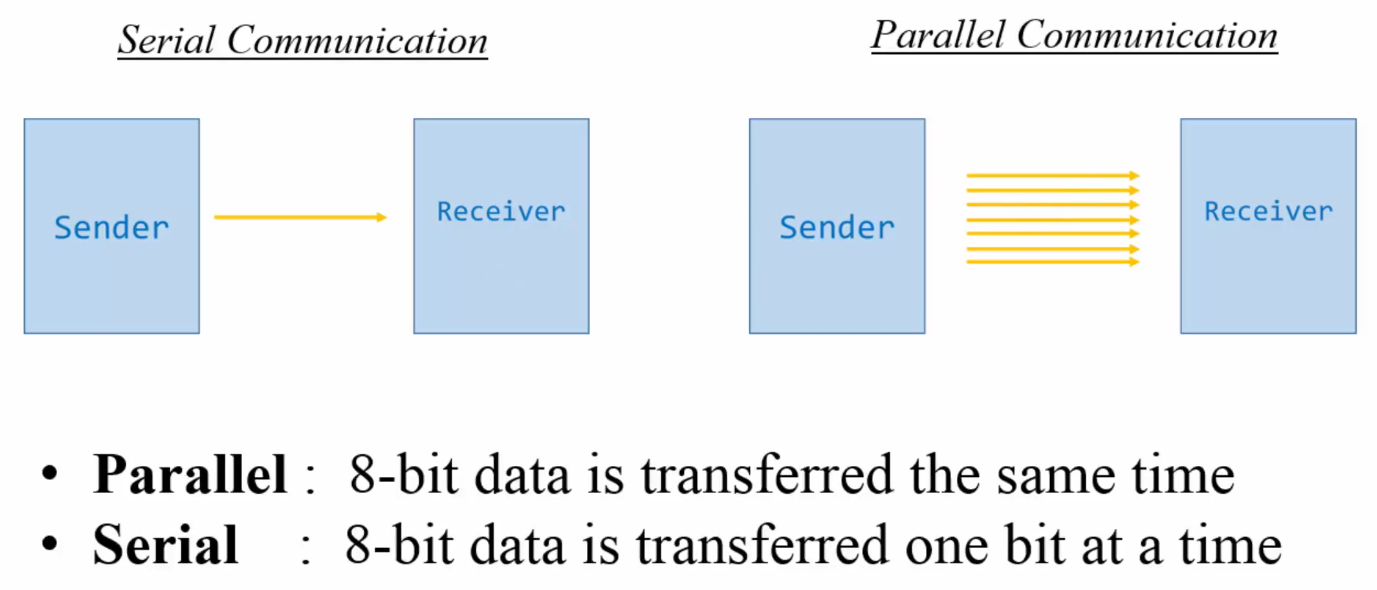
\includegraphics[scale=0.3,frame]{Figures/UART/com_type}
\caption{Serial vs parallel communication}
\label{fig:UART:com_type}
\end{figure}

\begin{itemize}

\item  Serial: 1 bit at a time $\leftrightarrow$ hence 1 arrow

\item  Parallel: multiple bits at a time $\leftrightarrow$ hence multiple arrow

\end{itemize}

\item Serial communication comes in 2 methods:

    \begin{enumerate}
    \item Synchronous: communication is via a clock

    \item  Asynchronous: no clock is used $\leftrightarrow$ Rx and Tx make convention about the baude rate
    
    \end{enumerate}

\item \underline{Transmission mode:}

In \autoref{fig:UART:mode_tx_rx}, we have all the transmission mode associated with some block diagram to illustrate the particular mode

\begin{figure}[h]
\centering
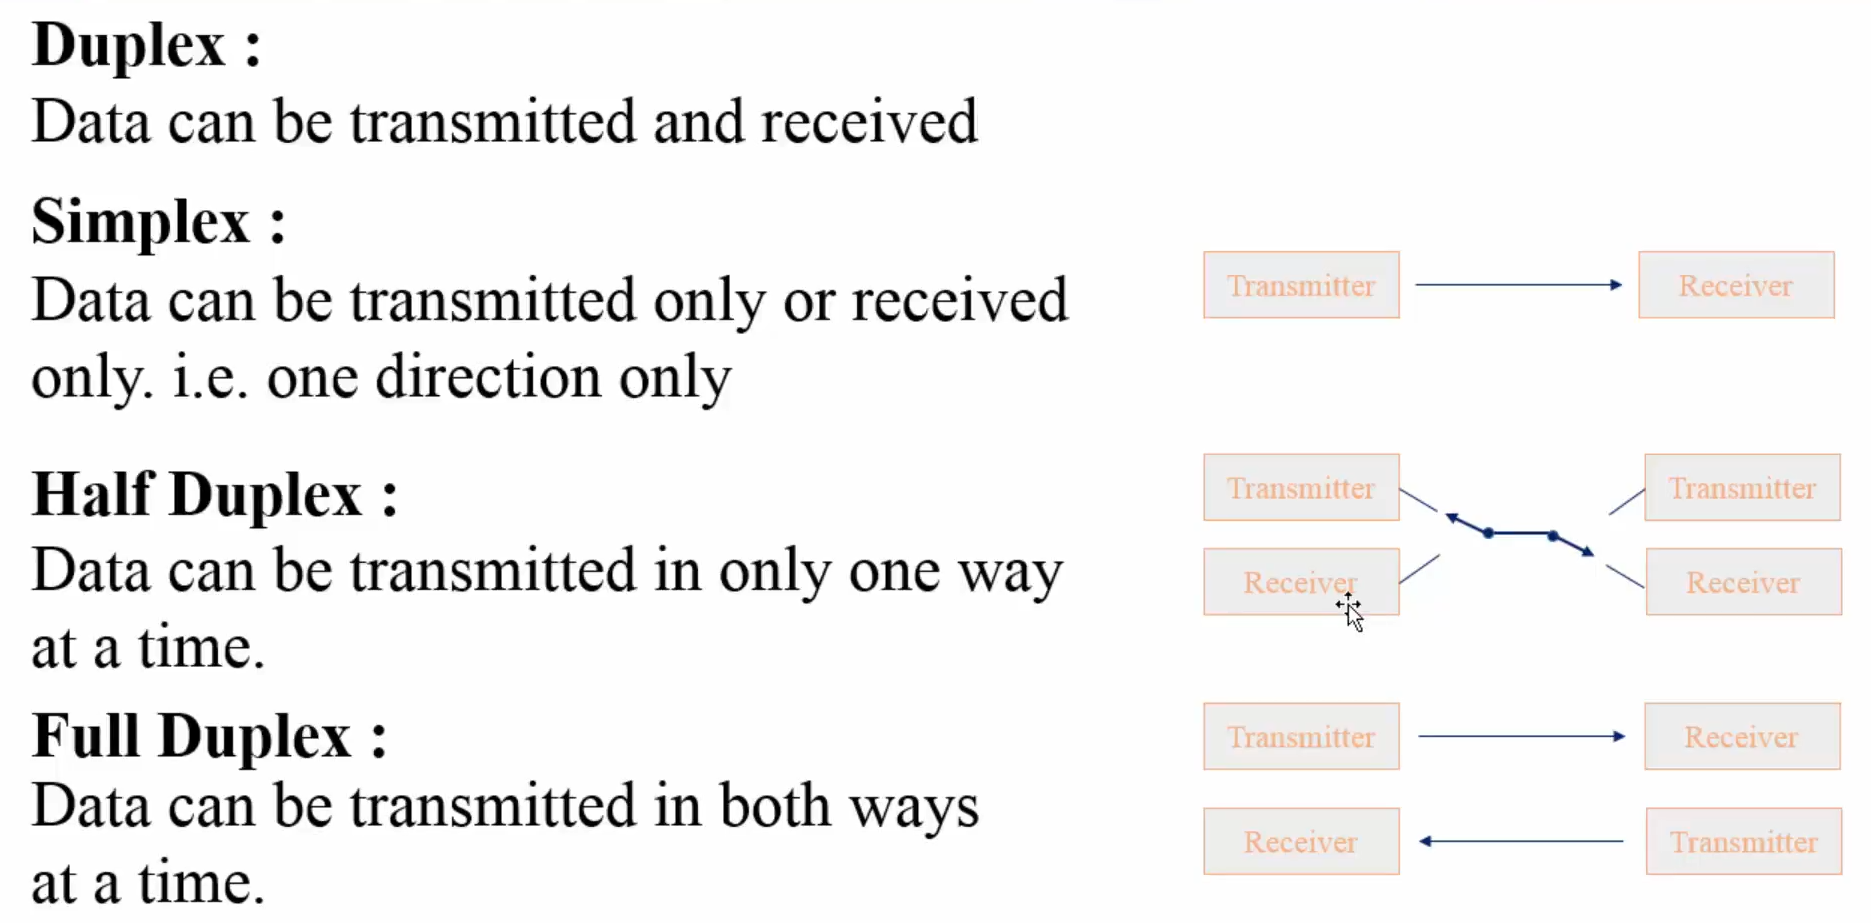
\includegraphics[scale=0.25,frame]{Figures/UART/mode_tx_rx}
\caption{Different transmission mode between a Tx and a Rx}
\label{fig:UART:mode_tx_rx}
\end{figure}

 \begin{itemize}
     \item the duplex is the general mode, where we have 2 possibility: either half duplex (data can be sent or received in only way), or full duplex (sent and receive in the same time)

    \item simplex is only in 1 direction: either transmit or receive
     
 \end{itemize}

\newpage
\item \underline{Protocol aspect:} 

\autoref{fig:UART:protocol_example} presents an example for sending the character \verb|A|, where beside the actual data, we use \tbi{start bit} and \tbi{stop bit}

\begin{figure}[h]
\centering
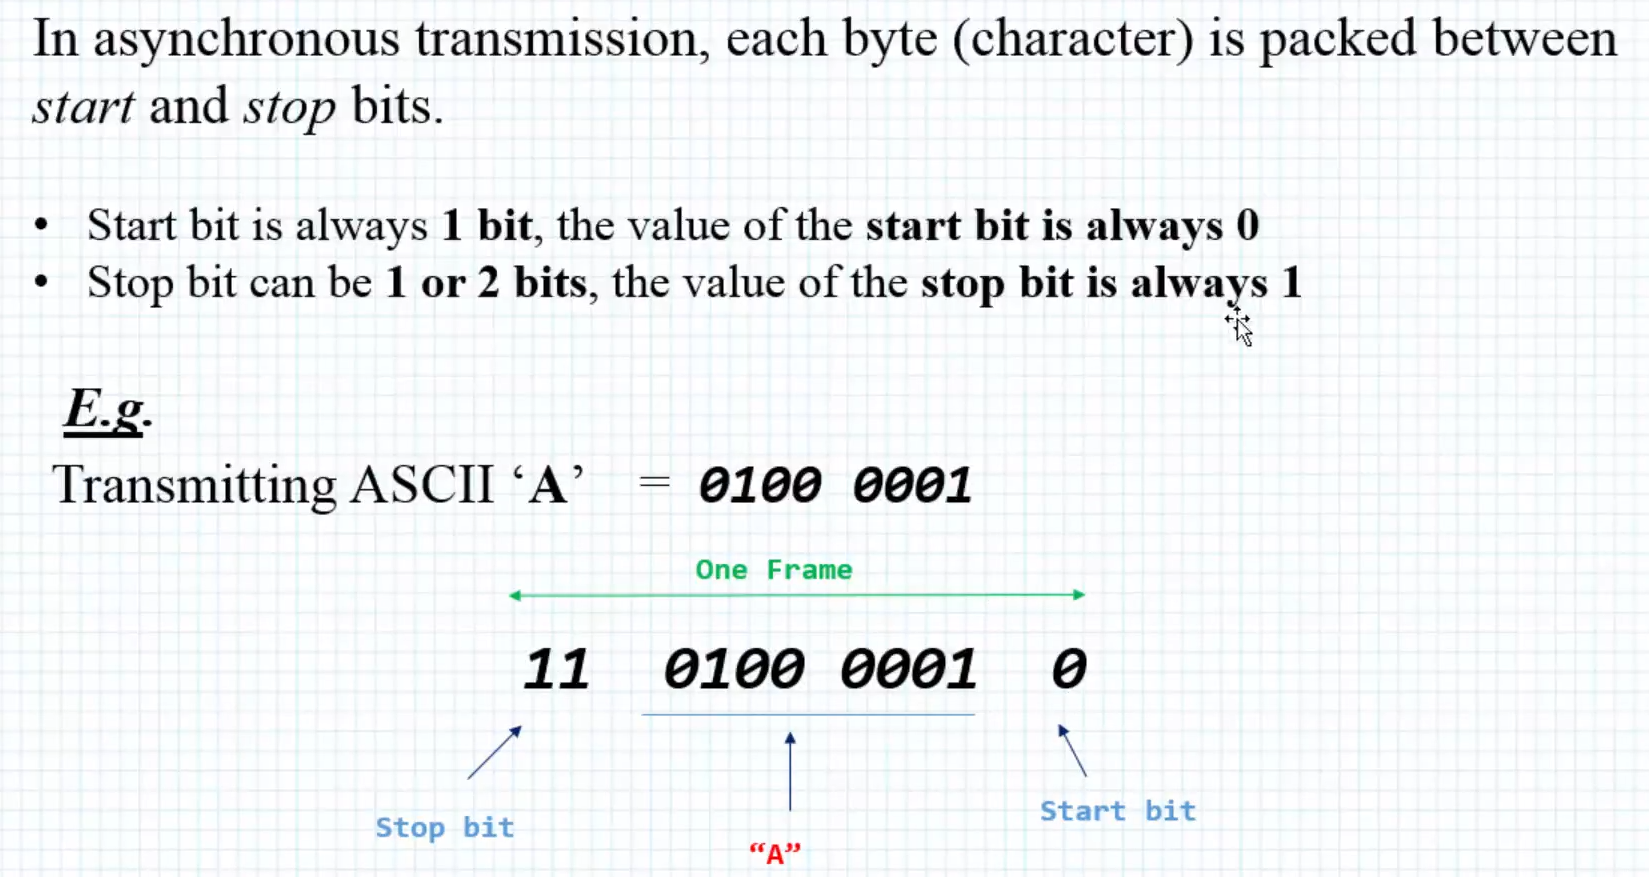
\includegraphics[scale=0.25,frame]{Figures/UART/protocol_example}
\caption{Protocol Example: start and stop bit}
\label{fig:UART:protocol_example}
\end{figure}

\item \underline{Some other configurations:}

There are also some other miscellaneous configuration 

    \begin{itemize}
    
    \item Word length: the number of data bits that can be transmitted or received. Can be 8 or 9 bits

    \item  Mode: Specify whether the Rx or Tx mode is enabled or disabled 
    
    \item Parity: for error checking, it comes with even or odd mode.
    
    \end{itemize}


\end{enumerate}


\newpage
\section{Coding Example}

$\mathrm{1}^\mathrm{st}$ in order to begin codning with UART, we need to see how many UART module we have in our board. To see that, we open the data sheet on the general block diagram (Figure 3 page 16).\\

We can see that we have 2 USART module: 1 connected to APB1 bus (named \verb|USART2|), and the others are connected to APB2 bus (named \verb|USART1| and  \verb|USART6|).\\

We are going to use the \verb|USART2| module, because it is connected to a USB port which we can use to communicated to our computer.\\


\underline{Note for hardware connection:}

\begin{itemize}

\item In stm32F411 nucleo board, it happens that the \verb|USART2| module is connected to the USB port in which we use to flash the firmware of the microcontroller.

\item In discovery board for example, the \verb|USART2| module is not connected to the USB port, so we need some converter device to make the USART $\rightarrow$ to USB conversion.

\todo{UART and Connection} \underline{\textit{UART and Connection}:} \textit{To explore this point later when re-working later with the discovery board} 


\end{itemize}

\subsection{UART Clock Registers Configuration}

\verb|USART2| module is connected to APB1 bus, which is handled by the \verb|RCC_APB1ENR| register.\\

In the reference manual (section 6.3.3 page 118), the bit number 17 is responsible for \verb|USART2| module.

\subsection{Pins Configuration}
\label{Sub:UART:Pins_Conf}

\verb|USART2| module has a Tx and Rx pins. To know to which GPIO these pins correspond, we open the data sheet to Table 9, the alternate function mapping page 48.\\

\underline{Description and Reading of the table:}

\begin{itemize}


\item The $\mathrm{1}^\mathrm{st}$ column contains all  ports and pins

\item  The element of the table contains some modules, such as USART-Tx, USAR-Rx,...

\item  When we scan for USART2-Tx, USAR2-Rx pins, we see that USART2-Tx corresponds to PA2 and USAR2-Rx corresponds to PA3.

\item  Also, USART2-Tx and USART2-Rx are in the AF07 column, and we will use that later.

\end{itemize}

\subsection{Alternate function register}

For Tx application for USART-2 module, we can see that until now we have:

    \begin{itemize}
    \item  Tx pin corresponds to PA2, and under AF7
    \end{itemize}

To set the alternate function value, there are 2 register responsible for that: GPIOx-AFRL, which handles the $\mathrm{1}^\mathrm{st}$ 8 I/O pins (pins 0 $\rightarrow 7$), and GPIOx-AFRH which handles the rest (pins 8 $\rightarrow 15$)

PA2 is the $\mathrm{2}^\mathrm{nd}$ pin under GPIO-A, so we need to configure GPIOx-AFRL.\\

\underline{Structure of GPIOx-AFRL:}

In the reference manual page 161, we see that GPIOx-AFRL is numerated AFRL0 $\rightarrow$ AFRL7. This means, for example, AFRL0 is for pin 0, AFRL1 is for pin 1, and so on.\\

In our case, we need to set AFRL2 (because we use PA2) to 0111 (which corresponds to Af7).\\

\underline{Programming Note:}

    \begin{itemize}
    
    \item In the header files provided by stm, we don't have GPIOA$\rightarrow$AFRL. Instead, we have GPIAO$\rightarrow$AFR[], where AFR is an array of size 2. 

    \item  GPIAO$\rightarrow$AFR[0] is for AFRL and GPIAO$\rightarrow$AFR[1] is for AFRH
    
    \end{itemize}

\newpage
\section{Summary UART}

\begin{itemize}

\item UART Tx and Rx pins mapping to GPIO: we use the alternate function mapping table, in page 48 in the data sheet (see \ref{Sub:UART:Pins_Conf}).


\end{itemize}


\end{document}

